\title{Event-Driven Architecture}
\author{Richard Thomas}
\date{\week{6}}

\maketitle

\section{Introduction}\label{sec:intro}

Event-driven is an asynchronous architectural style.
It reacts to events, which is different to the common procedural flow of control of many designs where messages are sent as requests.
It is a distributed event handling system, which is conceptually similar to event handling used in many graphical user interface libraries.

Events provide a mechanism to manage asynchronous communication.
An event is sent to be handled, and the sender can continue with other tasks while the event is being processed.
If necessary, an event handler can send an asynchronous message back to an event initiator indicating the result of the event processing.

Each event handler can be implemented in its own independent execution environment.
This allows each type of handler to be easily scaled to handle its load.
Asynchronous communication means that event generators do not need to wait for the handler to process the event.
Handlers can generate their own events to indicate what they have done.
These events can be used to coordinate steps in a complex business process.

\begin{figure}[h!]
    \begin{adjustwidth}{-10mm}{-10mm}
        \centering
        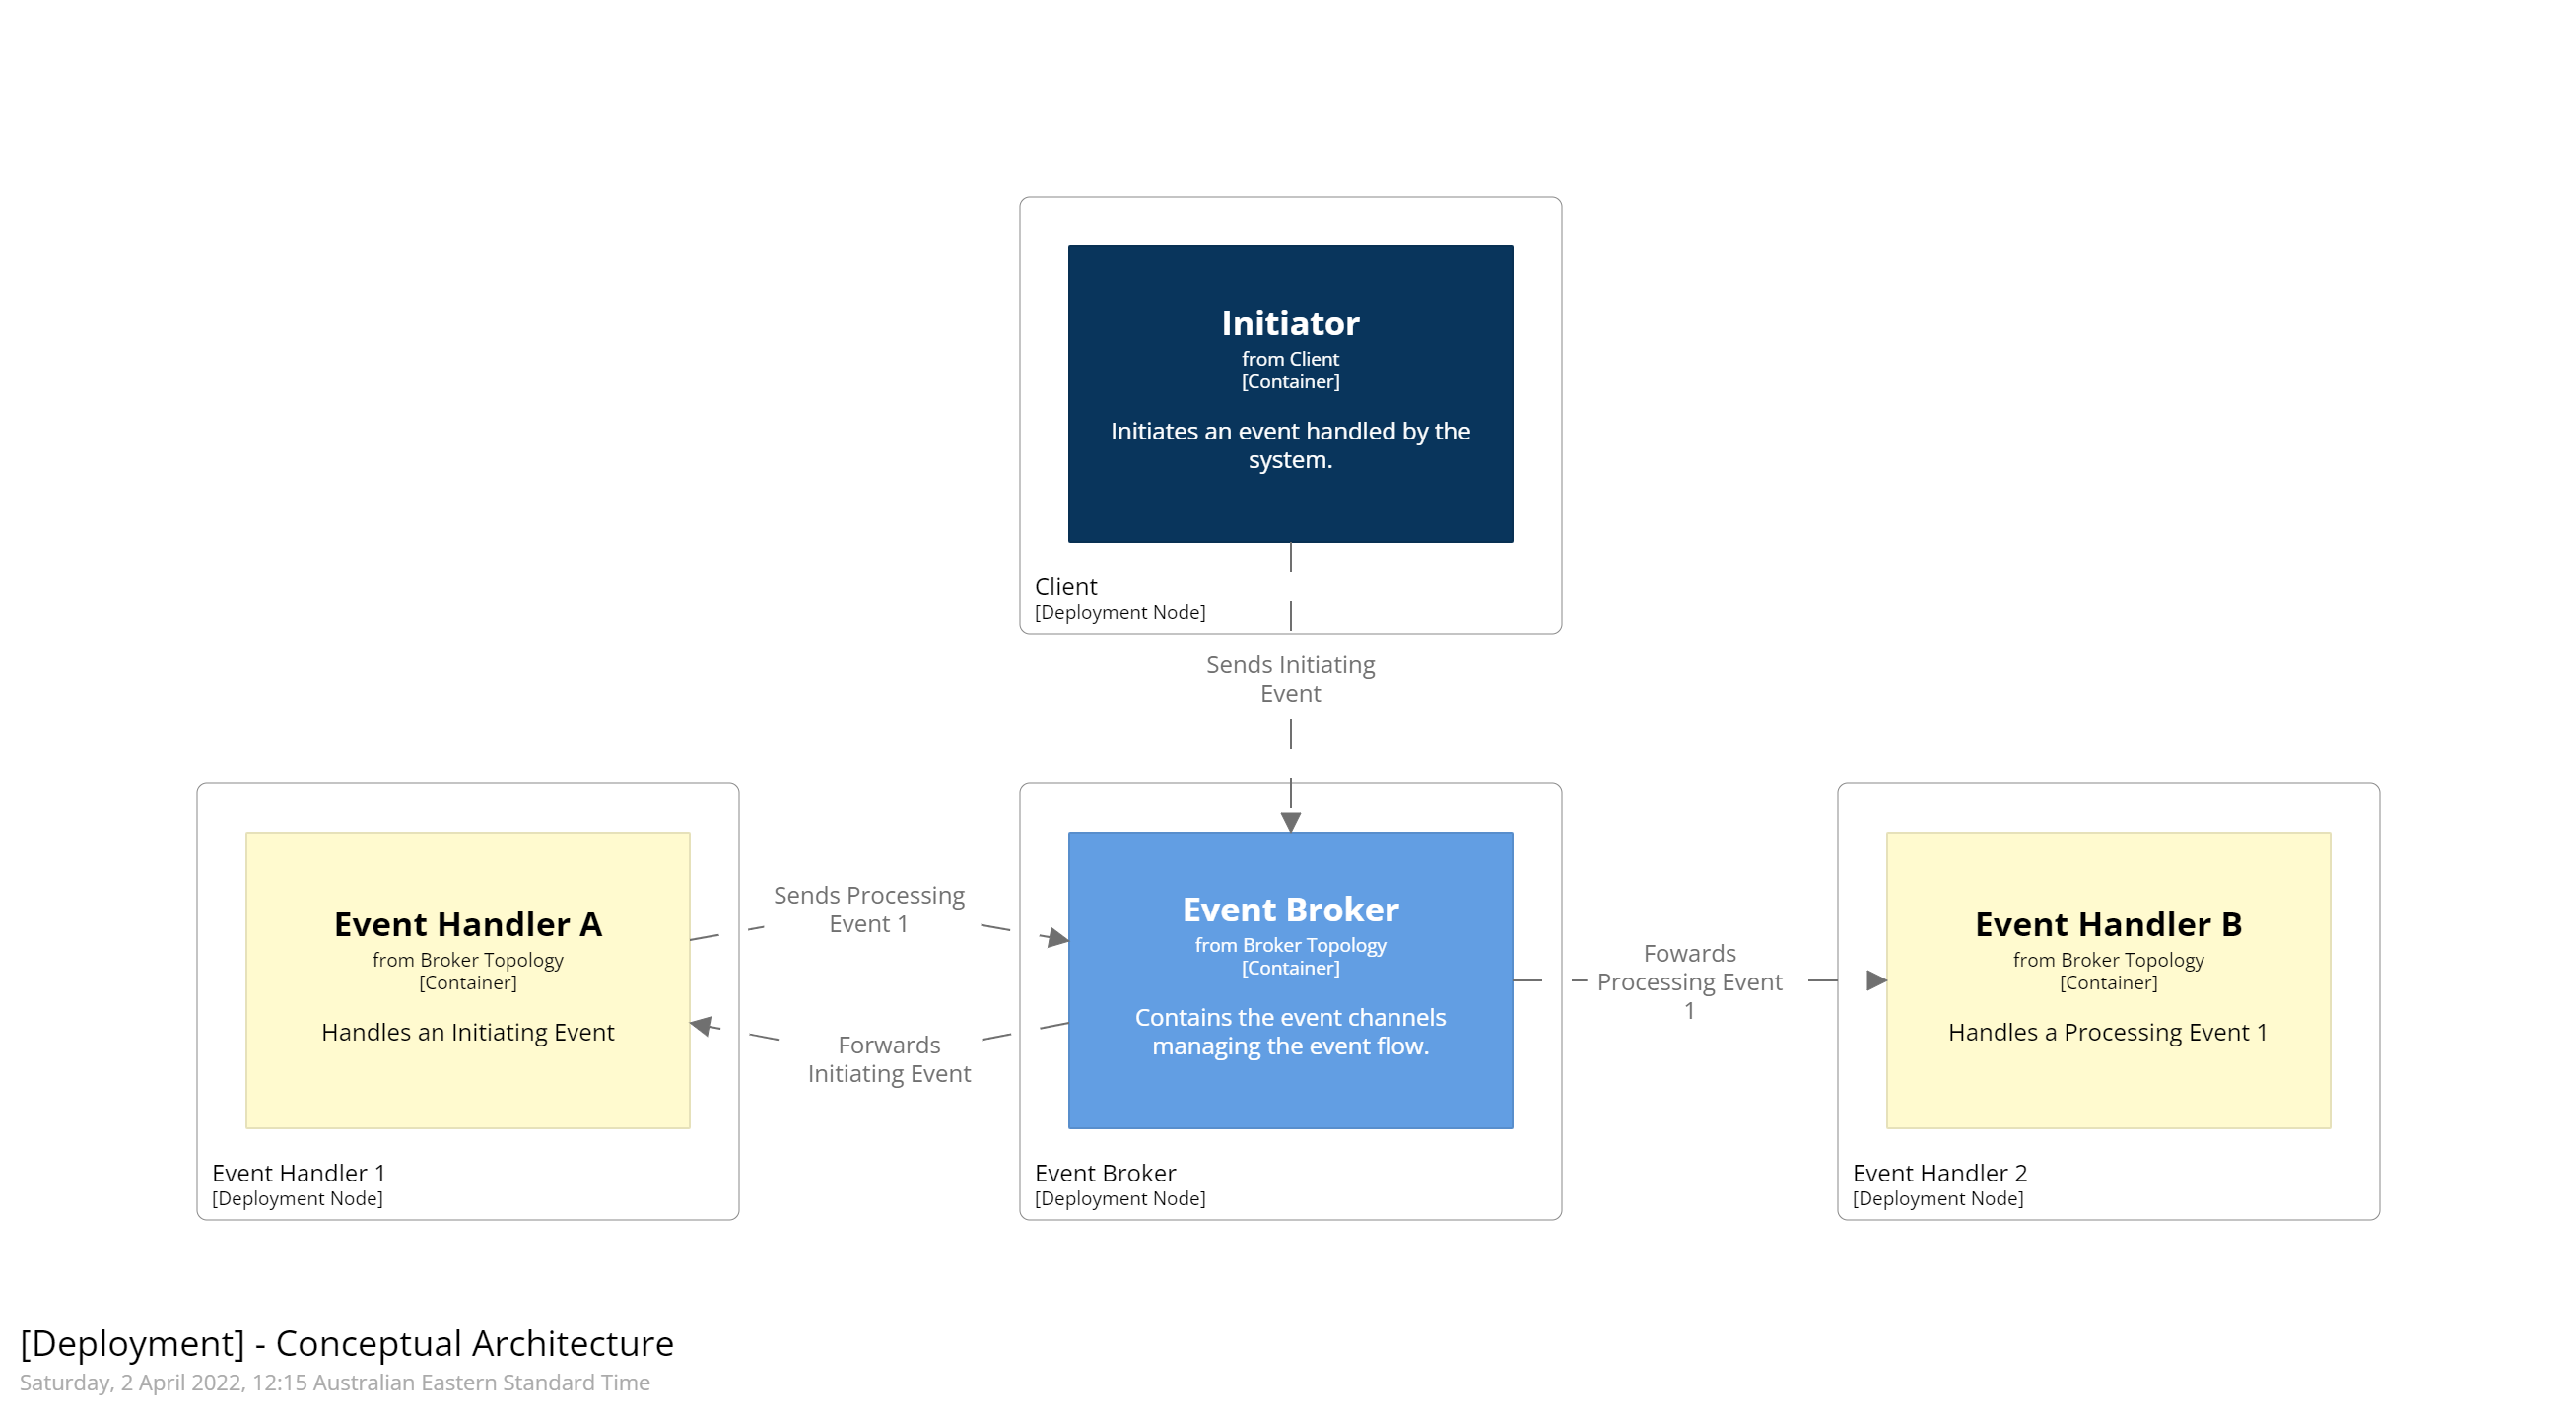
\includegraphics[trim=195 195 195 195,clip,width=0.95\paperwidth]{diagrams/conceptual-architecture.png}
    \end{adjustwidth}
    \caption{Conceptual deployment structure of an event-driven architecture.}
    \label{fig:conceptual-architecture}
\end{figure}

Figure \ref{fig:conceptual-architecture} shows the conceptual structure of an event-driven architecture.
A client of some form sends the initiating event to a central event broker or mediator.
That event is picked up by an event handler that processes the event.
That may lead to the event handler generating a processing event to move to the next step of the process.
The processing event is sent to the central broker and is picked up by another event handler.
This continues until the business process is completed.

An auction system, as shown in figure \ref{fig:auction-architecture}, could be implemented as an event-driven architecture.
\begin{itemize}[nosep]
    \item When a customer bids on an item, they initiate a bid \emph{event}.
    \item Upon receiving the bid event, the event broker notifies the bid handler which checks the bid against the current high bid and determines the new high bid.
    \item The bid handler generates a new high bid event.
    \item The event broker notifies the page update handler, which sends the new high bid to all pages displaying the item.
    \item The bid notification handler is also notified of the high bid event and it sends an email to the bidder with the result of their bid.
    \item The rebid notification handler is also notified of the high bid event.
             If the previous high bidder is no longer the high bidder, they are sent an email asking if they would like to make another bid.
\end{itemize}

\begin{figure}[h!]
    \begin{adjustwidth}{-10mm}{-10mm}
        \centering
        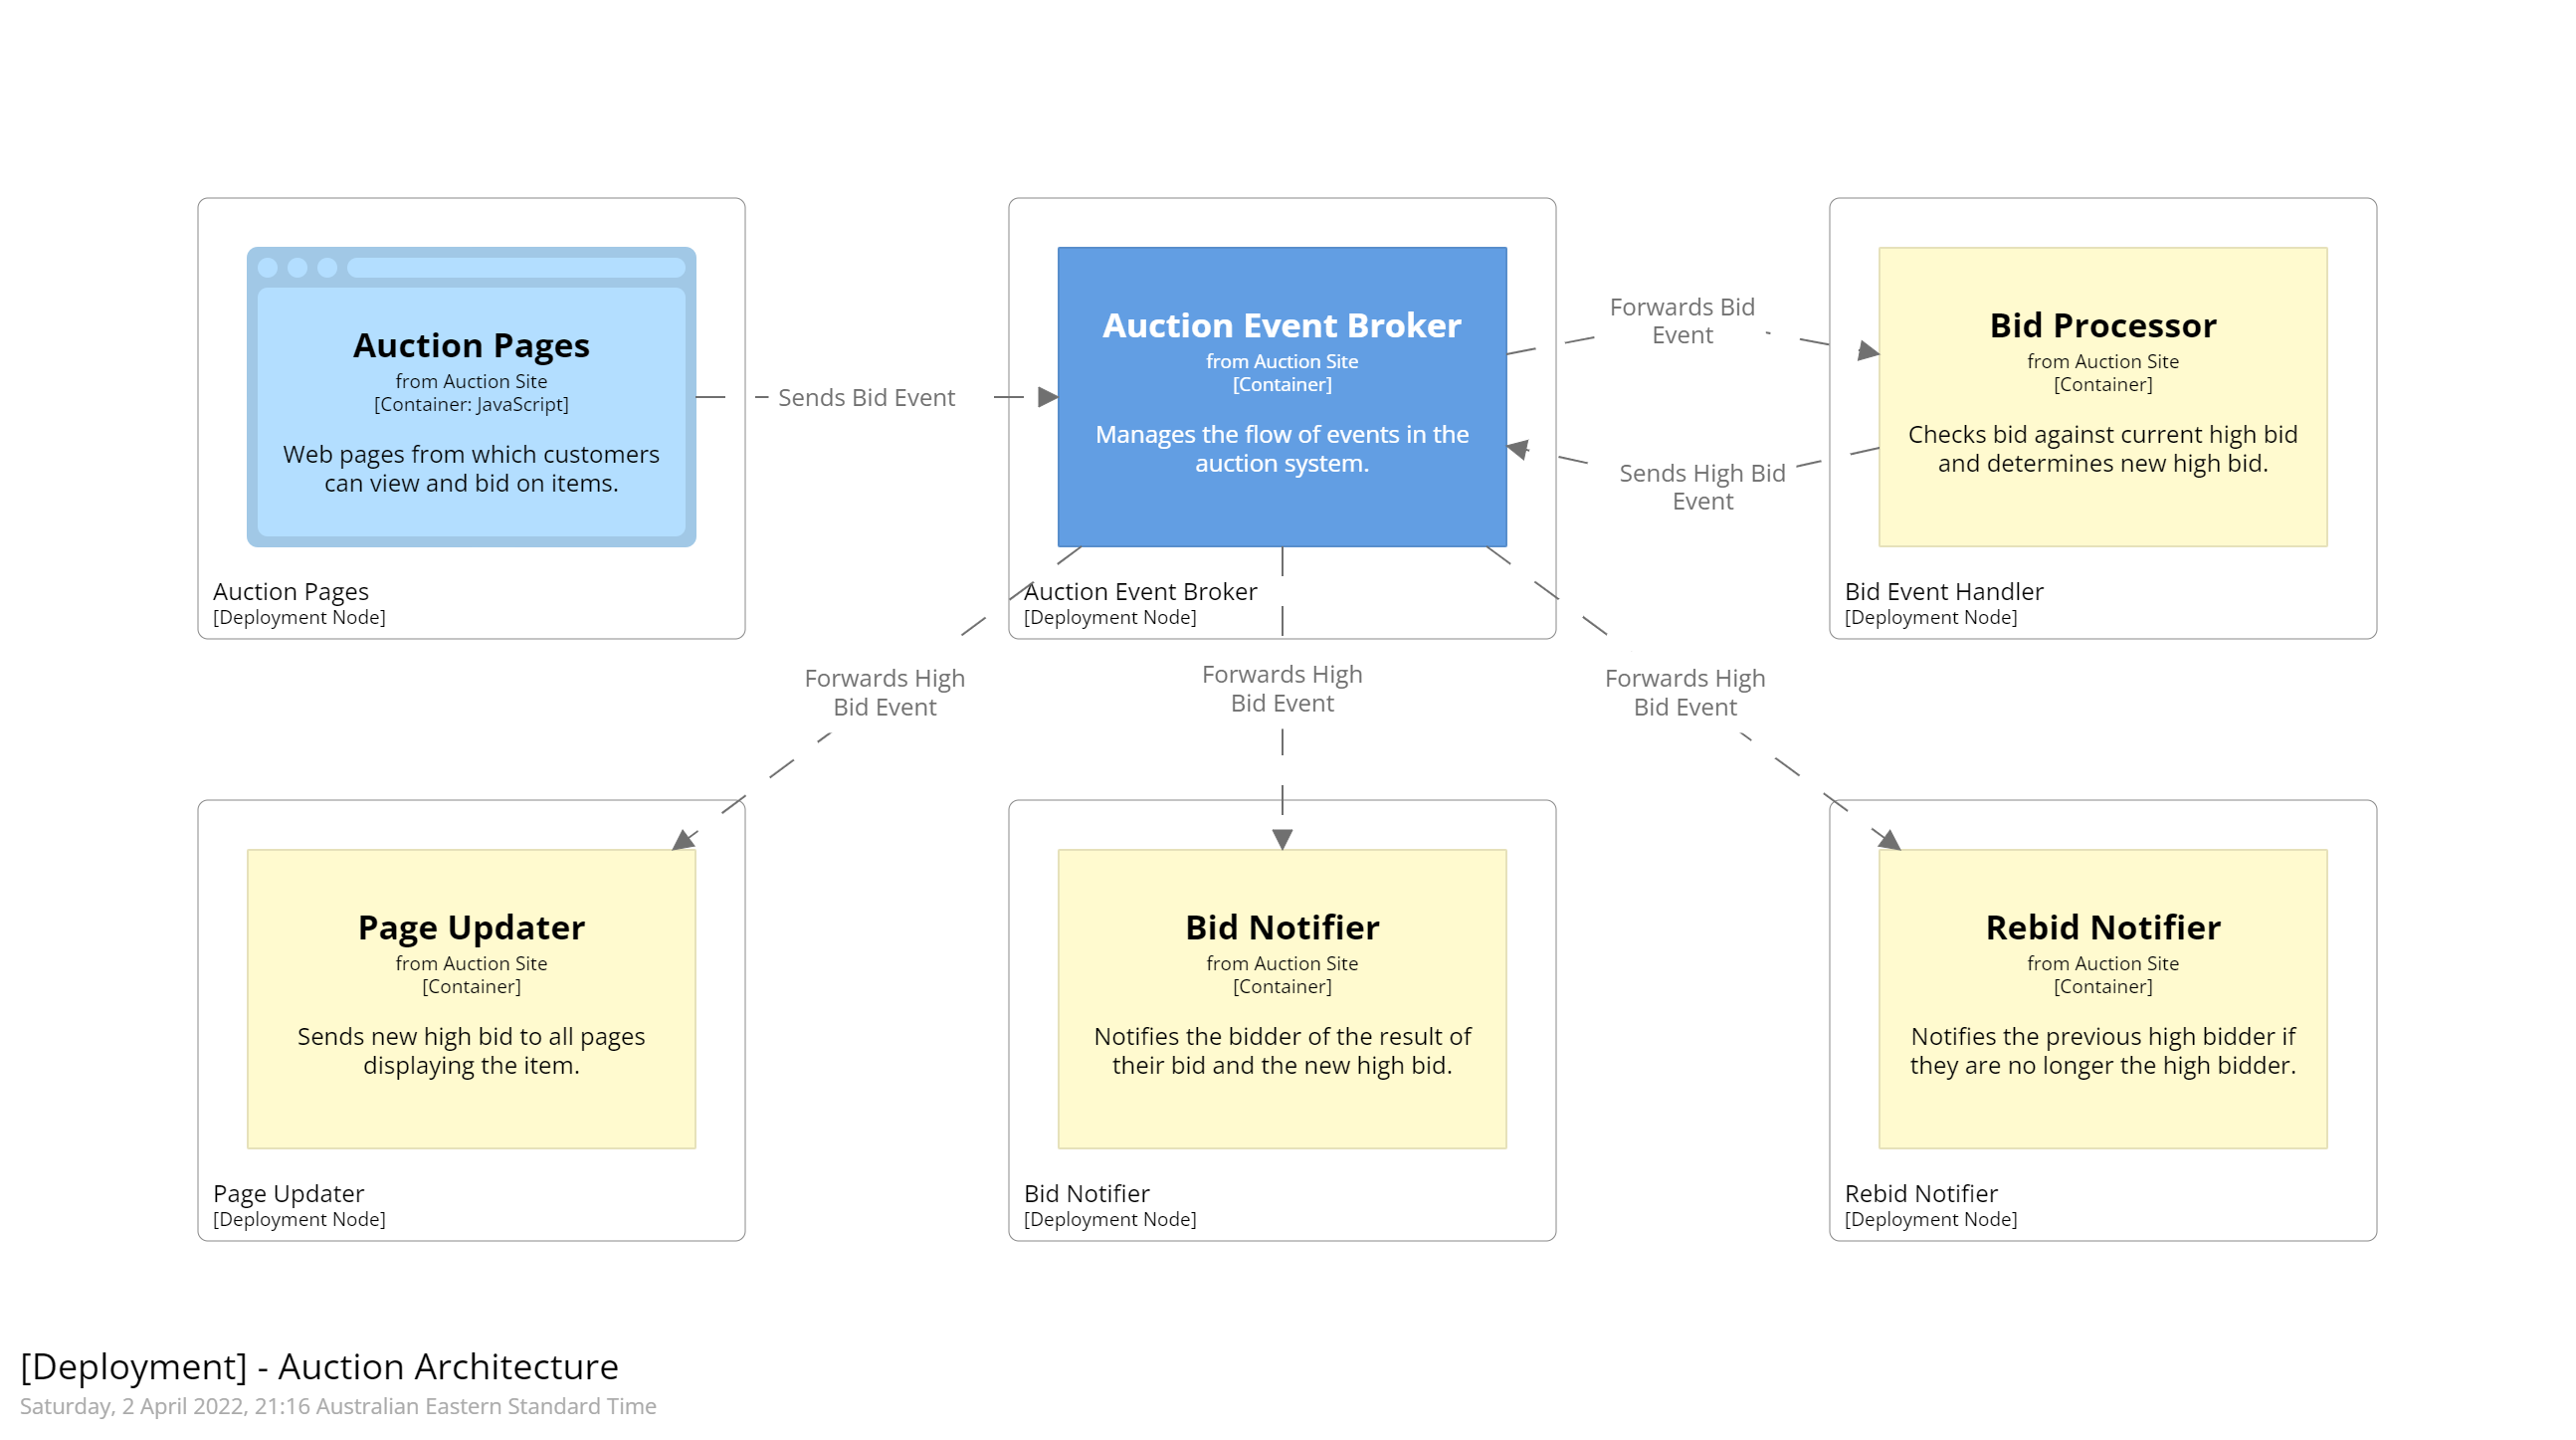
\includegraphics[trim=195 195 195 195,clip,width=0.95\paperwidth]{diagrams/auction-architecture.png}
    \end{adjustwidth}
    \caption{Auction bidding example event-driven architecture.}
    \label{fig:auction-architecture}
\end{figure}

There are two basic approaches to implementing an event-driven architecture.
They have different high-level structures or \emph{topologies}.
The \emph{broker topology} is the simpler of the two and is optimised for performance, responsiveness, scalability, extensibility, and low coupling.
The \emph{mediator topology} is more complex but is designed to provide reliability, process control, and error handling.


\section{Broker Topology}

The broker topology consists of five elements.

\begin{description}
    \item[Initiating Event] starts the flow of events.
    \item[Event Broker] has \emph{event channels} that receive events waiting to be handled.
    \item[Event Channel] holds events waiting to be processed by an event handler.
    \item[Event Handler] accepts and processes events.
    \item[Processing Event] sent by an event handler when it has finished processing an event.
\end{description}

% Possibly extend the auction example to make this more concrete?
% It will need to show events being ignored by system, and handlers not sending events at the end of processing.
\begin{figure}[h!]
    \begin{adjustwidth}{-10mm}{-10mm}
        \centering
        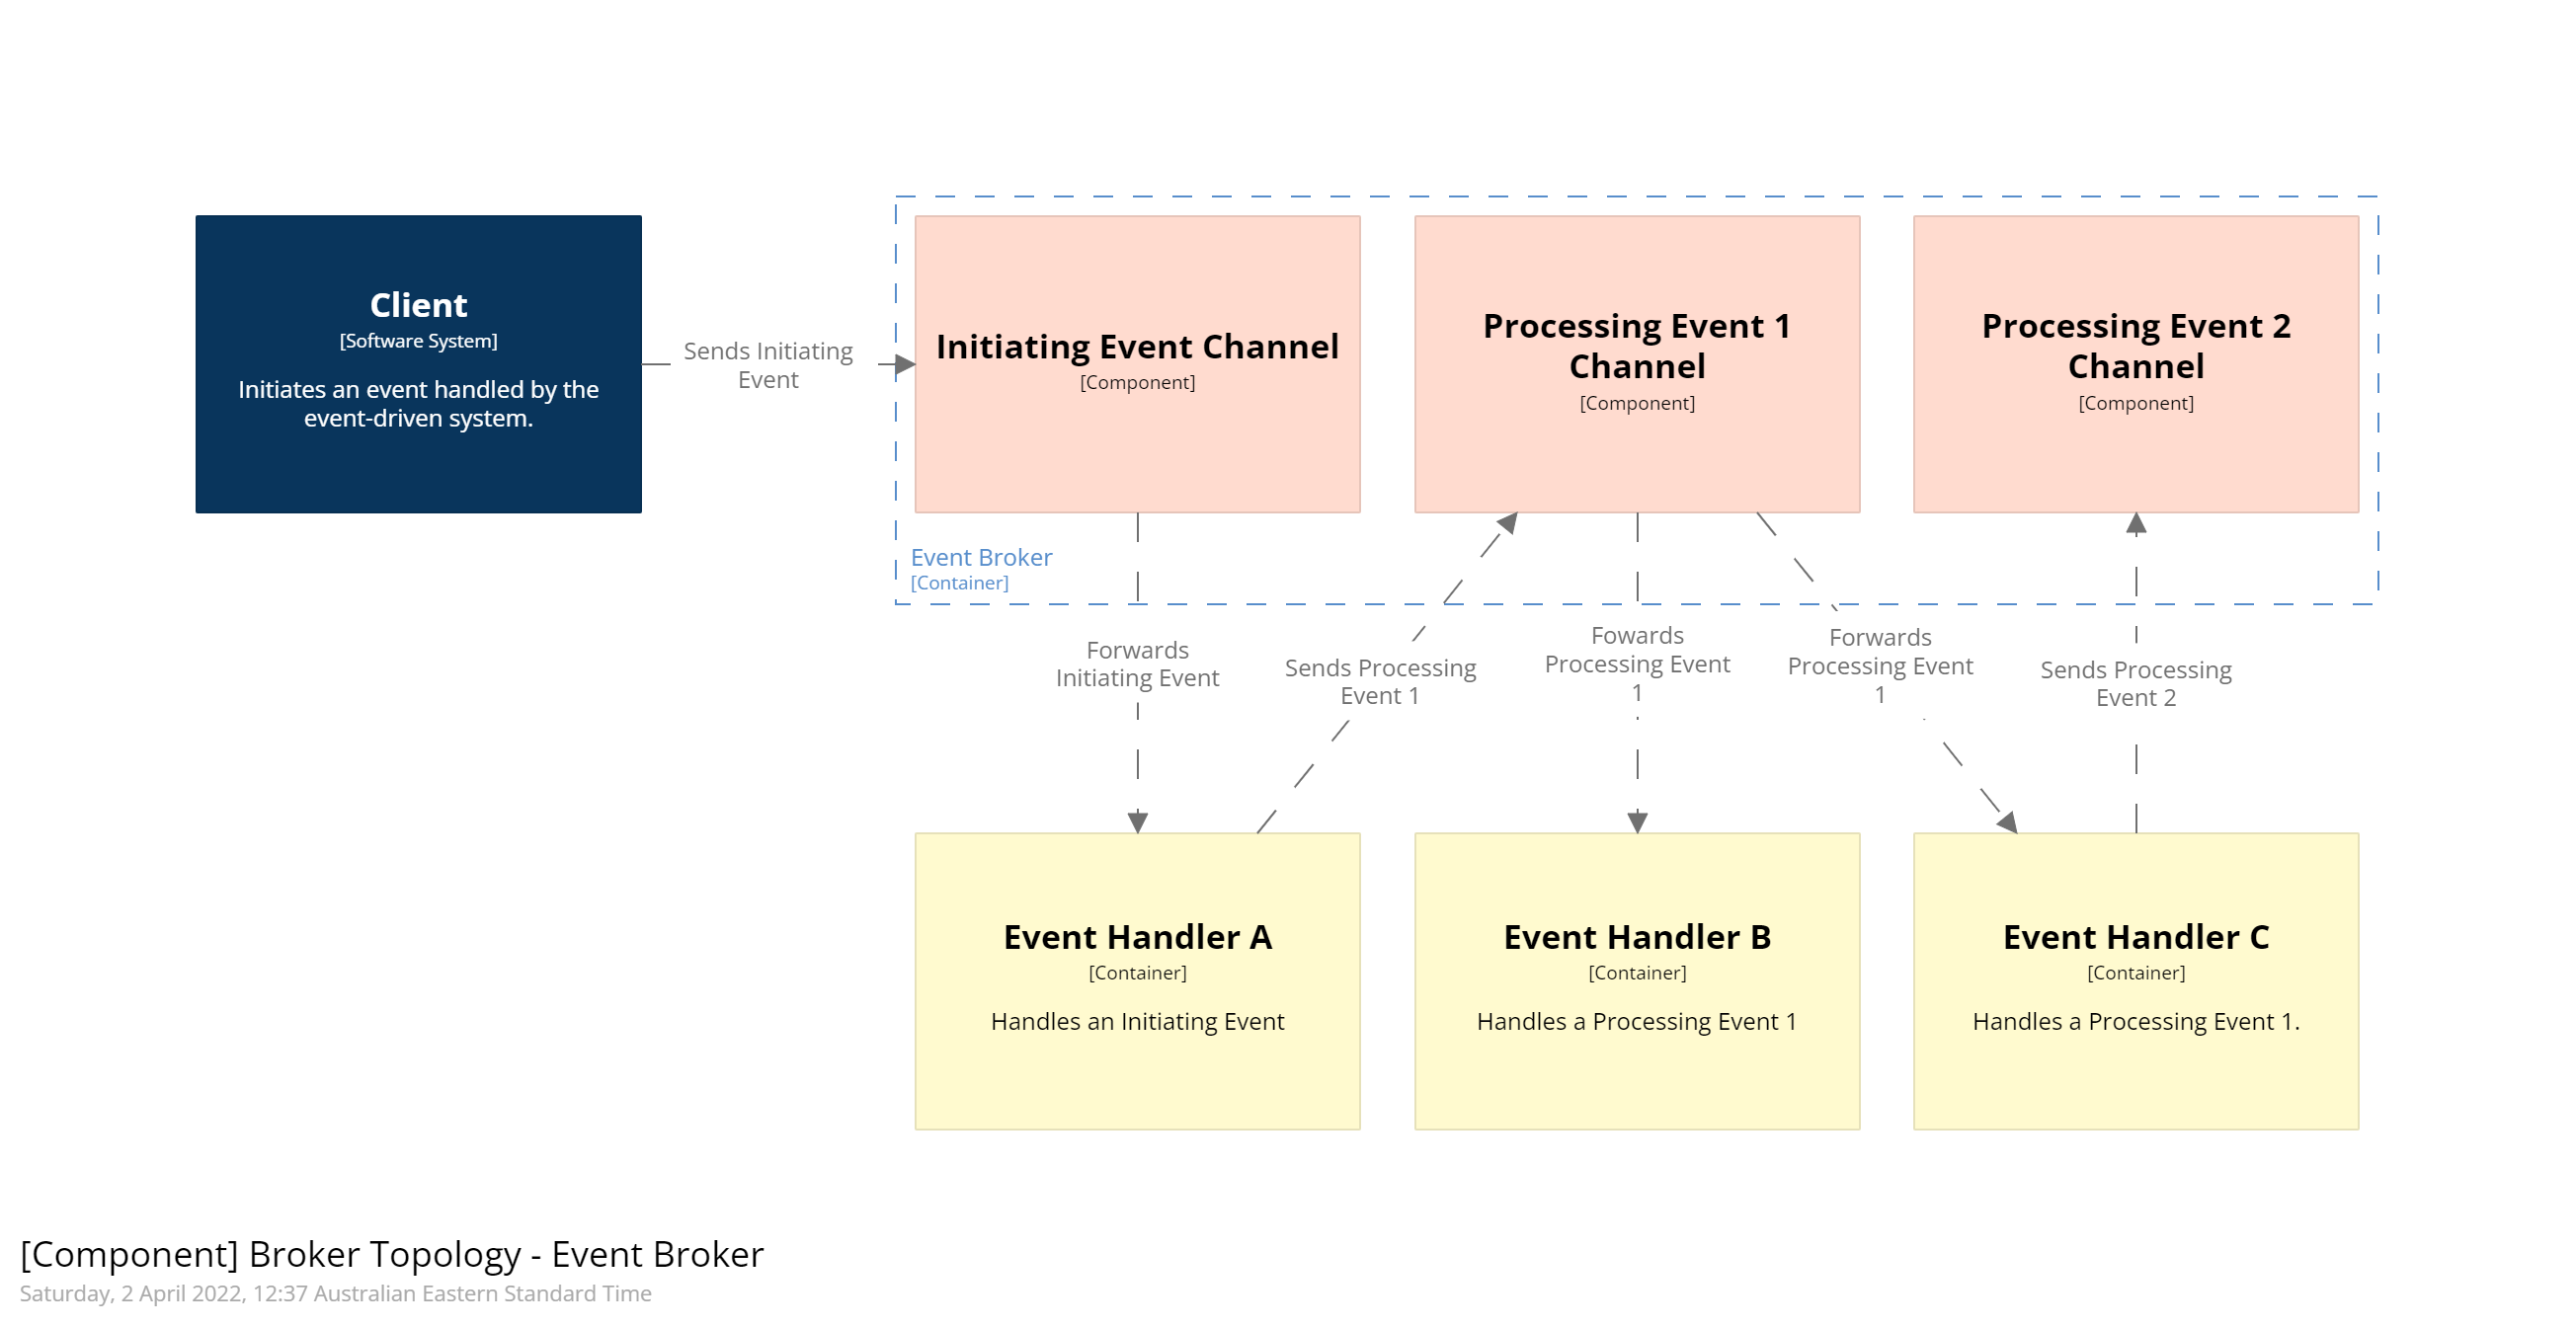
\includegraphics[trim=195 195 195 195,clip,width=0.97\paperwidth]{diagrams/broker-components.png}
    \end{adjustwidth}
    \caption{Basic broker topology.}
    \label{fig:broker-components}
\end{figure}

In figure \ref{fig:broker-components}, the \emph{Client} sends the \emph{Initiating Event} to the \emph{Initiating Event Channel} in the \emph{Event Broker}.
\emph{Event Handler A} accepts the event and processes it.
Upon completion of handling the \emph{Initiating Event},
\emph{Event Handler A} sends \emph{Processing Event 1} to the appropriate channel in the event broker.
\emph{Event Handlers B} and \emph{C} accept this processing event and perform their actions.
When \emph{Event Handler C} finishes processing it sends \emph{Processing Event 2} to its channel.
No event handler is designed to accept \emph{Processing Event 2}, so it is ignored.

Different event channels in the event broker provide a simple mechanism to coordinate the flow of events in a business process.
As shown in figure \ref{fig:broker-components}, there is a separate channel for each type of event.
This allows event handlers to register to be notified of only the type of events they can process.
This reduces the overhead of broadcasting events to handlers that cannot process them.
The consequence is that event sources need to send their events to the correct channel.
For a simple broker topology, this could be by sending event messages directly to a channel
or, for better abstraction and reduced coupling, the event broker may implement a façade that directs events to the correct channel.

\vspace{1mm}
\begin{definition}[Event Handler Cohesion Principle]\label{def:cohesion}
    Each event handler is a simple cohesive unit that performs a single processing task.
\end{definition}

The \emph{event handler cohesion principle} minimises the complexity of each handler,
and improves the ability of the system to scale only the tasks that need additional computing resources.
It also makes it easier to design each handler to be independent of the other handlers, reducing overall system coupling.

\subsection{Extensibility}\label{sec:extensibility}

There may be multiple event handlers for a single type of event,
shown by \emph{Processing Event 1} being sent to both \emph{Event Handler B} and \emph{C} in figure \ref{fig:broker-components}.
This allows more than one action to be performed when an event is sent.
This means that new event handlers can be added to the system as it evolves.
A new feature can be added by implementing an event handler to do something new when an event is received by the event broker.

In figure \ref{fig:broker-components}, when \emph{Event Handler C} finishes processing its event it sends \emph{Processing Event 2} to the event broker.
The diagram indicates that the system does not handle the event.
The purpose of doing this is to make it easier to extend the system.
Currently, the system may not need to do anything when \emph{Event Handler C} finishes processing,
but because it sends an event to indicate it has finished it means other tasks can be added to the system following \emph{Event Handler C}.
Because event handlers are independent of each other, \emph{Event Handler C} does not need to be modified to cater for this later addition of functionality.

If there are events that are not handled by the system, the event broker façade can ignore them, it does not need a channel to manage them.
If the system is extended and needs to process one of the ignored events, the event broker can create a new channel to manage them.

\emph{Event Handler B}, in figure \ref{fig:broker-components}, does not send an event when it finishes processing the event it accepted.
This is a valid design choice when implementing the system,
if there is nothing foreseeable that might need to know when \emph{Event Handler B} is finished processing.
The drawback is that if the system later needs to do something else when \emph{Event Handler B} is finished,
it will need to be modified to send an event to the event broker.
The tradeoff is reducing asynchronous communication traffic with unnecessary events, versus providing easy extensibility later.

\subsection{Scalability}

As was described in section \ref{sec:intro}, the broker topology is optimised for performance.
Each event handler is a separate container that can be deployed independently of other handlers.
A load balancer and an automated scaling mechanism ensures that each event handler can scale to manage its load.

There may be multiple clients sending events to be processed,
and each event handler may itself be a source of events.
This requires the event broker and its channels be able to handle the event traffic load.
The event broker itself can be deployed on multiple compute nodes, with its own load balancing and auto-scaling.
The challenge is to implement this in such a way that the event handlers do not need to know about the event broker's deployment structure.

A simple distributed event broker could deploy each channel on a separate compute node.
The event broker façade is deployed on its own node and manages receiving events and sending them to the appropriate channel.
The façade also manages how event handlers register to receive notification of events from channels.
This works until the event traffic to the façade or a single channel exceeds their capacity.

A more robust approach, which scales to very high traffic levels, is to federate the event broker.
This allows the façade and channels to be distributed across multiple nodes
but provides an interface that the clients and event handlers can treat as a single access point.
The complexity of implementing a federated computing system is beyond the scope of this course.
There are several libraries (e.g. ActiveMQ or RabbitMQ)
and cloud-computing platforms (e.g. AWS SQS, AWS MQ or Google Cloud Pub/Sub) that provide this functionality.
They can still be used when the system does not need to scale to a federated event broker,
as they provide the underlying implementation for the event broker.

\subsection{Queues}

The other issue that the channels need to manage to allow scalability is holding events until they are processed by an event handler.
The simple approach is that a channel implements a queue.
Events are added to the end of the queue as they are received.
When an event reaches the front of the queue, all the event handlers for the channel are notified that the event is available.
The channel queue needs to be configured to cater for different implementation choices.
The simple option is that when an event handler accepts the event, it is removed from the queue.
This means that only one type of event handler listening to the channel will process the event.

If the system needs all the different types of event handlers to process the event,
the queue needs to be configured so that the event is not removed from the queue until all the event handlers have retrieved it.
This can be implemented in the queue by having multiple \emph{front of queue pointers}, one for each type of event handler listening to the channel.
This allows different event handlers to process through events in the queue at different rates.
The queue should be implemented to pass queue size or the amount of time events are in the queue to the auto-scaling mechanism for each event handler.
This can be used as part of the logic to determine when to deploy new event handlers, or to scale-back when traffic decreases.

To increase reliability, the queue can be implemented to only remove the event from the queue once the event handler has finished processing it,
rather than when it has been received by the handler.
This allows another event handler to process the event if the first event handler to accept the event fails.
A timeout mechanism can be used to provide this functionality.
If the queue does not receive notification that the event has been processed within a certain amount of time,
it notifies the event handlers that the event is available.

Another consideration to increase reliability is dealing with when the event broker, or one of its queues, fails.
If queues are implemented as in-memory queues, events in the queue will be lost when the event broker or queue fails.
Queues can be implemented to persistently store events until they have been processed.
A federated event broker will further improve reliability by making it less likely that a single queue will fail between receiving an event and storing it persistently.

\subsection{Streams}

An alternative to channels using queues to manage events is to use streams instead.
Event sources send events to the event broker and they are added to the appropriate stream.
Each channel becomes a stream and events are added to the stream.
The observer pattern is used where the channel is the subject and the event handlers are the observers.
When an event is added to a stream, the channel notifies all its observers that an event has been added.
The event handlers then decide whether to retrieve the event and process it.

The most important difference of using streams versus queues is that the events are stored permanently in the stream.
Event handlers can process events at their own pace.
Because the events are stored permanently, history is maintained.
This allows the system to go back and redo past processing or for an audit to be conducted of what happened during processing.

\subsection{Queues vs Streams}

Queues work well when there are known steps in the business process being implemented.
Queues ensure that all preceding events in the business process are completed before the next step.
Queues can ensure that events are only processed once (known as ``exactly once'' semantics).
An ecommerce website is an example of the type of system suited to using queues.
This is because there is a fixed set of rules about which event handlers process which events.

Streams work well when there are multiple event handlers responding to events,
particularly when event handlers may choose to ignore some events based on various conditions.
Streams mean that the event broker or channels do not need to be notified if an event handler wants to ignore an event.
Because streams store events permanently, data analysis of the system's behaviour can be done by processing past events.
Streams work well for social media platforms as monetisation of the platform depends on analysing user behaviour.
If user generated events are stored permanently in streams, new analyses can be performed on past data.

Streams also work well for \link{Internet of Things}{https://www.oracle.com/au/internet-of-things/what-is-iot/} (IoT) systems.
An IoT system may generate a vast number of events.
Streams make it more practical to process different events at an appropriate pace.
Some events may need almost immediate processing (e.g. a monitor reporting heart failure).
Other events may need periodic processing (e.g. analysing patient blood pressure over a period of time).
An IoT system may also have a large number of event handlers where some IoT devices process events.

Streams also enable \emph{event sourcing} as a persistence mechanism.
Event sourcing stores every event, and its associated state, rather than storing and updating system state.
This makes it easier to analyse how the system is used and what changes happen to the state over time.

% Add example broker-based event-driven architecture for Sahara.
%\subsection{Sahara Example}
%
%The service-based architecture example for the Sahara eCommerce system is designed to perform synchronous processing of requests.
%A customer \emph{requests} to view a product's details through a REST API and receives a response with the result.
%Similarly, a customer adding a product to their shopping cart is another request.
%
%Multiple customers could submit bids for the same item at almost the same time (e.g. bid sniping).
%These bid events are queued to be processed in the order they are received.
%This queuing mechanism allows event handlers to process messages that arrive faster than the handler can process them.
%It assumes that the message load will reduce in time and that the event handler will process all messages in the queue.


\section{Mediator Topology}

The mediator topology extends the broker topology by adding an \emph{event mediator}.
The event mediator manages the flow of events to implement the business process.
There are six elements that make up the mediator topology.

\begin{description}
    \item[Initiating Event] starts the flow of events.
    \item[Event Queue] holds initiating events sent to the event mediator.
    \item[Event Mediator] coordinates sending events to the event handlers to implement a business process.
    \item[Event Handler] accepts and processes events.
    \item[Event Channel] holds events waiting to be processed by an event handler.
    \item[Processing Event] sent by the event mediator to start the next step in the process.
\end{description}

\begin{figure}[h!]
    \begin{adjustwidth}{-10mm}{-10mm}
        \centering
        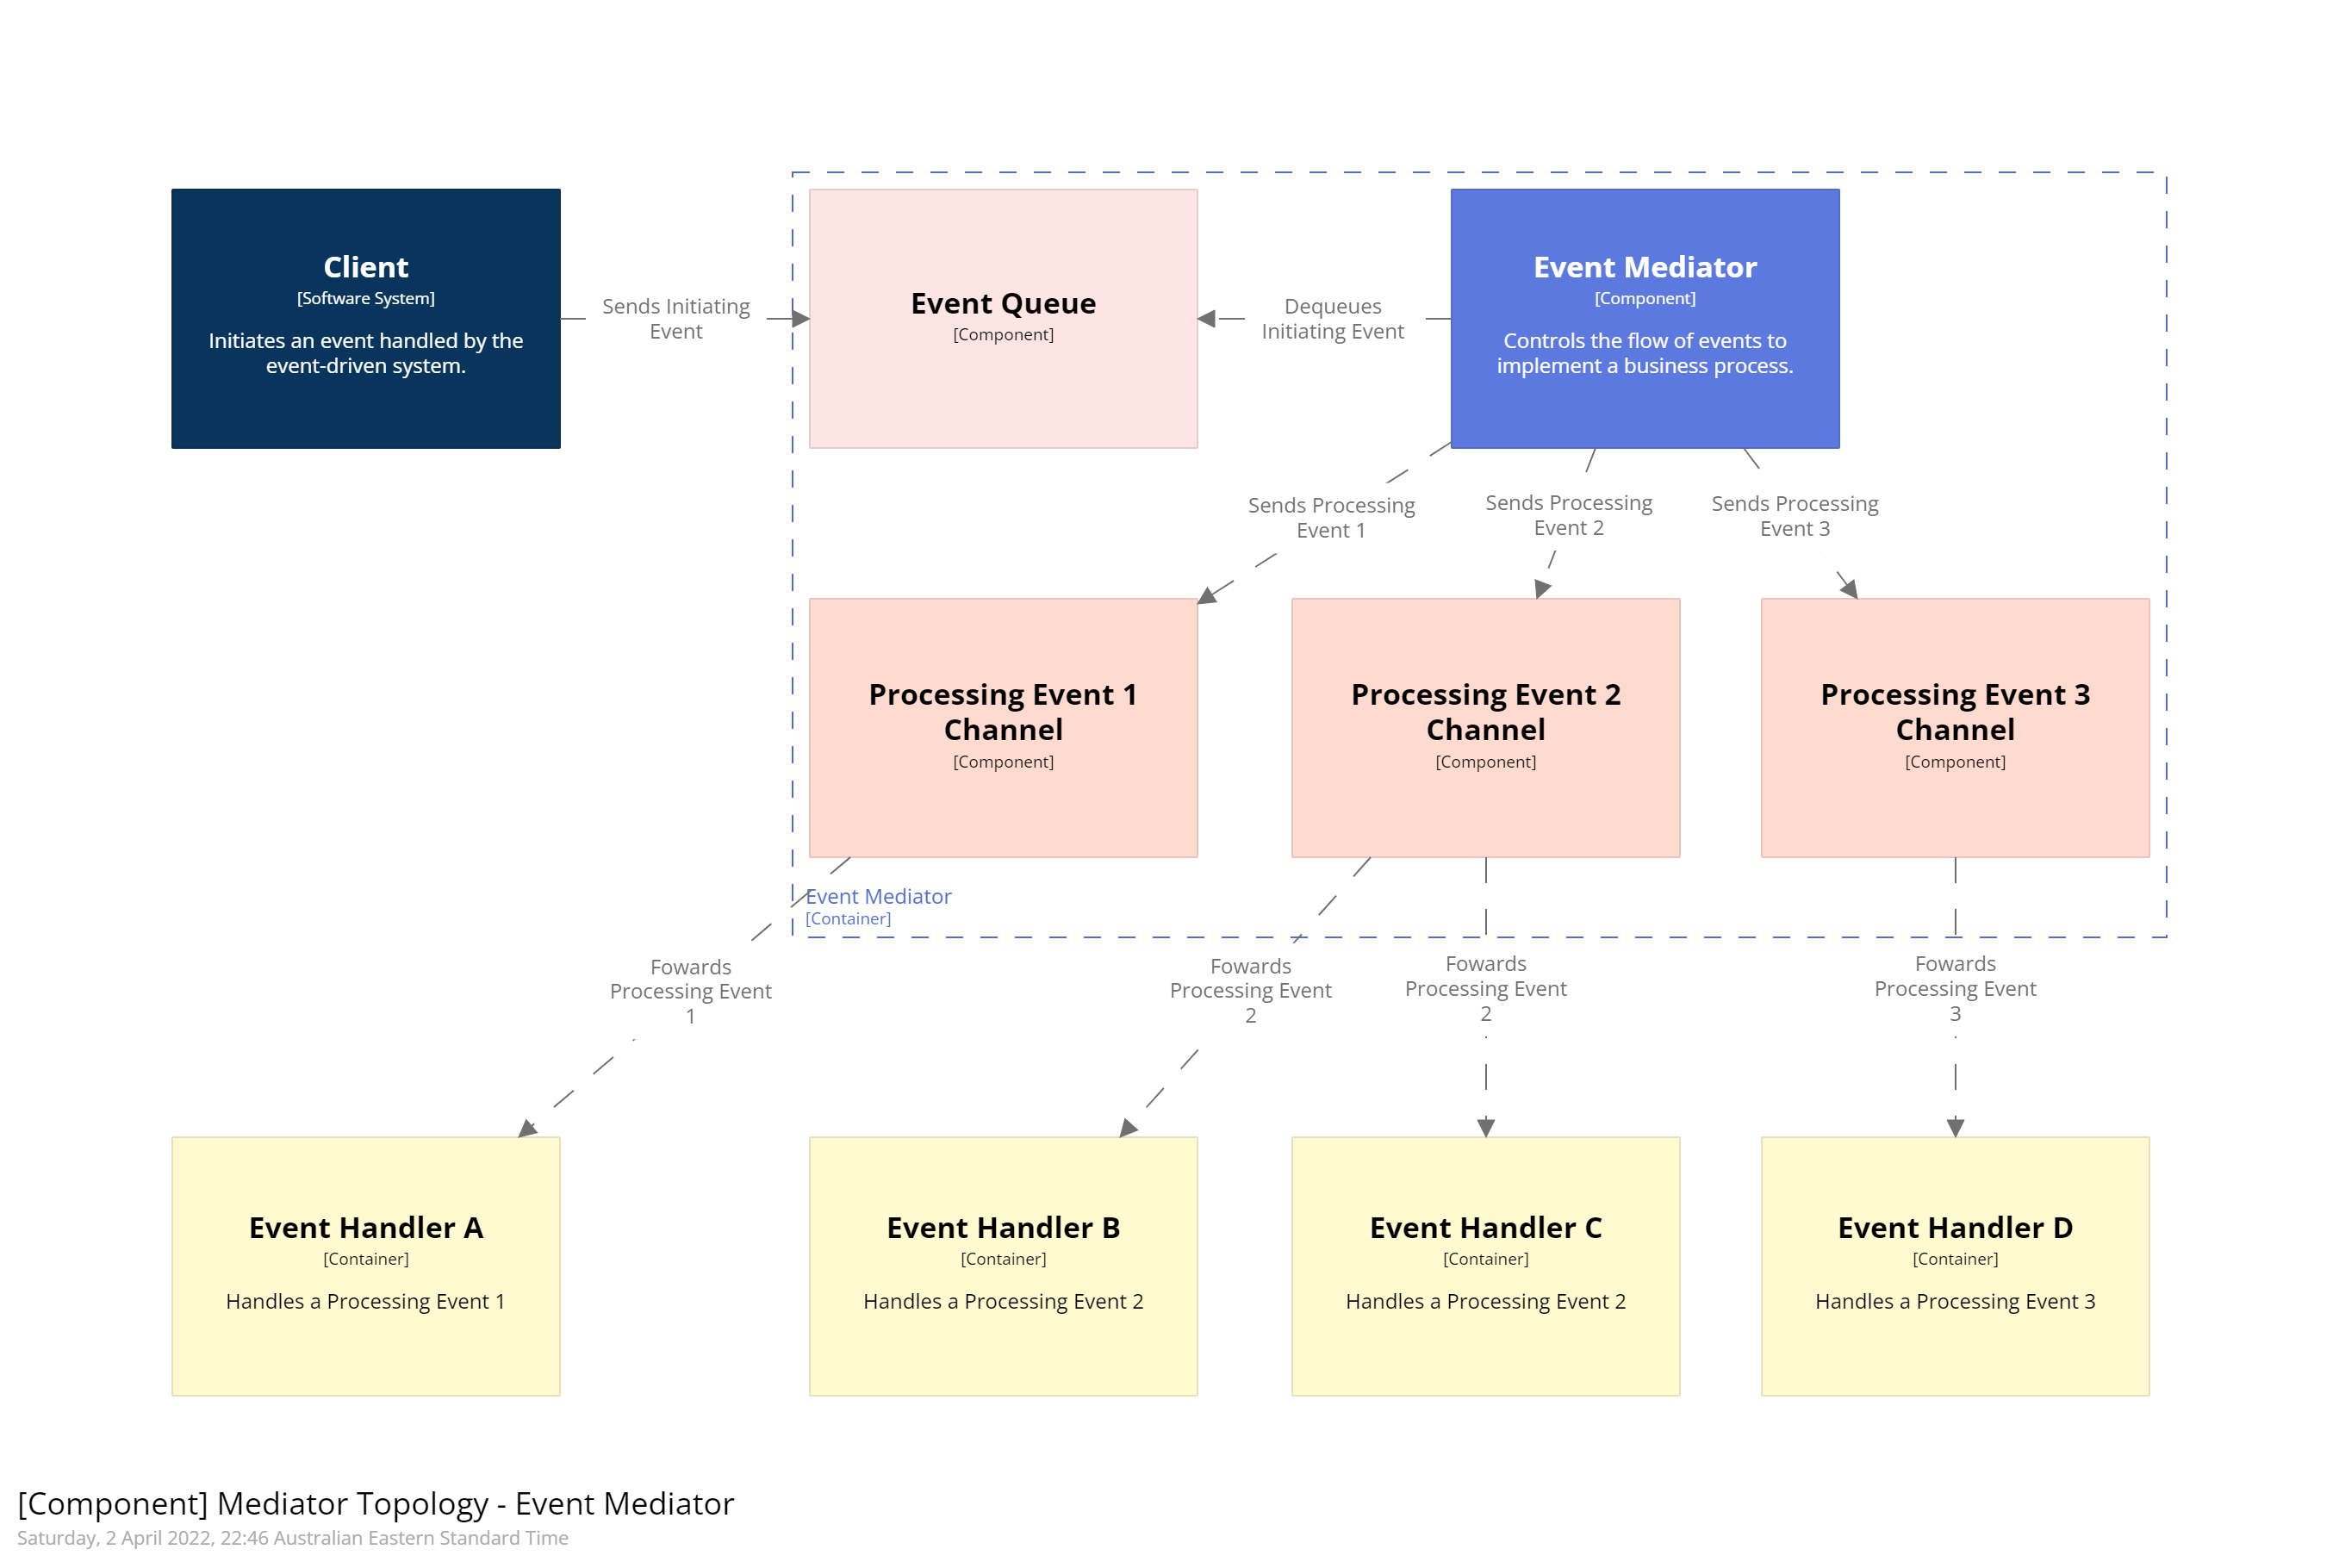
\includegraphics[trim=195 195 195 195,clip,width=0.97\paperwidth]{diagrams/mediator-components.png}
    \end{adjustwidth}
    \caption{Basic mediator topology.}
    \label{fig:mediator-components}
\end{figure}

In figure \ref{fig:mediator-components}, the \emph{Client} sends the \emph{Initiating Event} to the \emph{Event Queue}.
The \emph{Event Queue} notifies the \emph{Event Mediator} that an event has been enqueued.
The \emph{Event Mediator} dequeues the next \emph{Initiating Event} and starts the business process to deliver the behaviour for that event.
The \emph{Event Mediator} adds a \emph{Processing Event 1} to its channel.
The channel notifies the event handlers listening for this type of event.
The event handlers retrieve the event from the channel and process it.
When an event handler finishes processing it does not send a processing event to the \emph{Event Mediator} to be handled.
Rather, the event handler usually sends an asynchronous message to the \emph{Event Mediator} indicating that the handler has finished processing.
When the \emph{Event Mediator} receives a completion message from an event handler,
the mediator determines what is the next step in the process and sends a processing event to the appropriate channel to continue the logic.

The event mediator allows the system to implement more sophisticated logic to implement the business process.
Based on the result received from an event handler when it finishes processing an event,
the mediator can decide which processing event to send next.
This allows conditional or iterative logic to be implemented in the business process.
Unlike the broker topology, which only has a sequential flow through the business logic based on event handlers sending new events when they finish processing.


\section{Design Considerations}\label{sec:design-considerations}

A service-based architecture is typically used for medium-sized systems.


\section{Service-Based Principles}

There are a couple of principles which should be maintained when designing a service-based architecture
to produce a simple, maintainable, deployable and modular designs.

\vspace{1mm}
\begin{definition}[Independent Service Principle]\label{independent-service}
    Services should be independent, with no dependencies on other services.
\end{definition}



\section{Extensions}

There are a few common variations of the service-based architecture to consider.

\subsection{Separate Databases}

The first variation  we will consider is to have separate databases for each service.


\section{Conclusion}

Service-based architecture is an approach to designing a distributed system that is not too complex.
Domain services provide natural modularity and deployability characteristics in the architecture design.
Well designed service APIs improve the encapsulation and hide implementation details of the services.
